\documentclass[dvisvgm,border=2pt]{standalone}
% Shared by every figure. Two colours only: black becomes the text colour of
% whatever theme the app is in, and `accent` becomes the brand — see
% scripts/build-figures.mjs. Everything else is done with opacity.
\usepackage{amsmath}
\usepackage{amssymb}
\usepackage{tikz}
\usepackage{pgfplots}
\pgfplotsset{compat=1.18}
\usetikzlibrary{arrows.meta,positioning,calc,backgrounds,fit,patterns.meta}
\definecolor{accent}{RGB}{255,0,255}
\pgfplotsset{
  every axis/.append style={
    axis lines=left,
    axis line style={draw opacity=0.35},
    tick style={draw opacity=0.35},
    tick label style={font=\scriptsize,opacity=0.7},
    label style={font=\scriptsize,opacity=0.7},
    legend style={draw=none,fill=none,font=\scriptsize},
    every axis plot/.append style={line width=0.7pt},
  },
}
\tikzset{
  every picture/.style={font=\scriptsize},
  faint/.style={opacity=0.3},
  quiet/.style={opacity=0.55},
  box/.style={draw,opacity=0.35,rounded corners=2pt,inner sep=4pt},
  hot/.style={accent},
}

\begin{document}
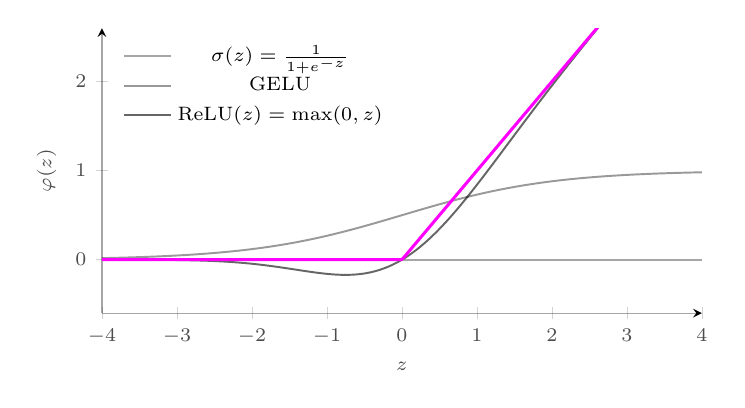
\begin{tikzpicture}
  \begin{axis}[width=9.2cm,height=5.2cm,
      xlabel={$z$},ylabel={$\varphi(z)$},
      xmin=-4,xmax=4,ymin=-0.6,ymax=2.6,
      ytick={0,1,2},
      legend style={at={(0.02,0.98)},anchor=north west}]
    \addplot[domain=-4:4,samples=2,opacity=0.35]{0};
    \addplot[domain=-4:4,samples=200,opacity=0.4]{1/(1+exp(-x))};
    \addlegendentry{$\sigma(z)=\frac{1}{1+e^{-z}}$}
    \addplot[domain=-4:4,samples=300,opacity=0.6]
      {0.5*x*(1+tanh(sqrt(2/pi)*(x+0.044715*x^3)))};
    \addlegendentry{GELU}
    \addplot[domain=-4:4,samples=300,accent,line width=1.1pt]{max(0,x)};
    \addlegendentry{$\mathrm{ReLU}(z)=\max(0,z)$}
  \end{axis}
\end{tikzpicture}
\end{document}
